\chapter{Analyse}
I projektets start blev der udarbejdet en analyse af systemet. I dette kapitel vil der blive beskrevet de valg, som blev taget til projektet. Den fulde analyse kan findes i bilag. \\

\section{Firebase}
	Til håndtering af back-end i systemet er der valgt, at bruge Firebase. Firebase\cite{Firebase} er en development platform som Google har udviklet. Firebase tilbyder flere forskellige funktionaliteter til både iOS og Android. \\
	Firebase er serverless, hvilket betyder at der ikke er behov for at opsætte en server til databasen, for at kunne interagere med databasen. Da Rambøll ikke en server tilrådig, så derfor virkede dette, som den optimale løsning. \\

\section{Xamarin}
	Applikationen udviklet til systemet, er blevet udviklet i Xamarin Forms\cite{Xarmain}. Dette er et cross platform udviklingsværktøj, som giver mulighed for at udnytte share code. Dette gør at man kan bruge samme kode til både iOS og Android platformen. \\
	Valget bag dette er et ønske fra Rambøll, som gerne ville have et system der både virkede på iOS og Android, da deres ansatte brugte begge styresystemer.
	
	\begin{figure}[H]
		\centering
		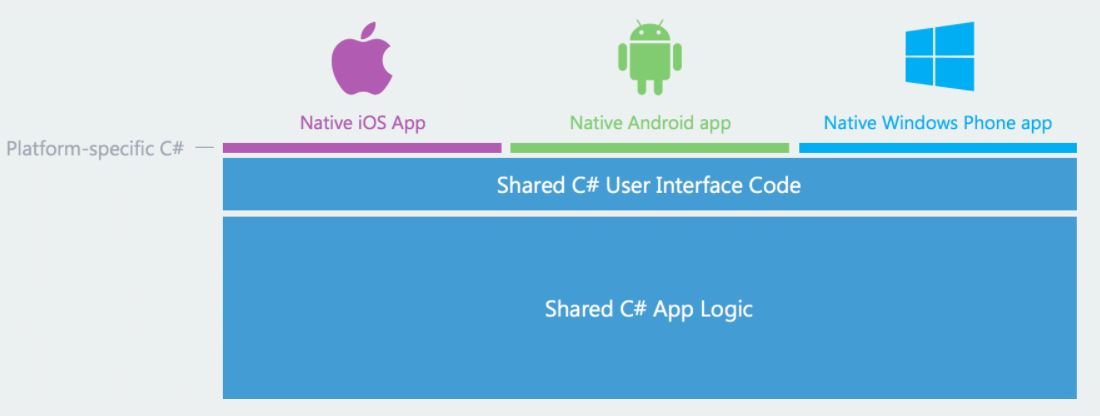
\includegraphics[width=1\linewidth]{Analyse/XarmarinShare}
		\caption{Kode deling i Xamarin Forms.\cite{Xarmain}}
		\label{fig:CodeShare}
	\end{figure}
	
	Fordelen ved Xamarin i forhold til andre cross platform værktøjer er, at det er en indbygget del af Visual Studio, som var programmet der blev brugt til udvikling af applikationen. \\
	Derudover kan der udviklet i C\#, som er et kodesprog der undervises i på skolen.